\documentclass[12pt]{article}

\usepackage[a4paper,margin=2.5cm]{geometry}
\usepackage{amsmath, amssymb, amsthm}
\usepackage{bm}
\usepackage{hyperref}
\usepackage{graphicx}
\usepackage{caption}
\usepackage{listings}
\usepackage{xcolor}
\usepackage{float}
\usepackage{placeins}
\graphicspath{{figures/}}

\lstdefinestyle{code}{
  basicstyle=\ttfamily\small,
  numbers=left,
  numberstyle=\tiny,
  numbersep=8pt,
  keywordstyle=\color{blue},
  commentstyle=\color{teal!70!black},
  stringstyle=\color{orange!70!black},
  showstringspaces=false,
  breaklines=true,
  frame=single,
  framerule=0.3pt,
  rulecolor=\color{black!15}
}
\lstset{style=code}

\title{Gaussian Mixture Model Tutorial}
\author{}
\date{\today}

\begin{document}
\maketitle

\section{Introduction}
Gaussian Mixture Models (GMMs) describe data as a weighted sum of multiple Gaussian components. Each component captures a latent cluster with its own mean, covariance, and mixing weight. GMMs excel at modeling elliptical clusters and overlapping distributions, offering richer shapes than K-means while retaining probabilistic assignments and density estimates.

\section{Theory and Formulas}
\subsection{Mixture Likelihood}
For observation \(\mathbf{x}\) in \(\mathbb{R}^d\), the mixture density is
\begin{equation}
p(\mathbf{x}\,|\,\Theta) = \sum_{k=1}^K \pi_k \mathcal{N}(\mathbf{x} \,|\, \bm{\mu}_k, \mathbf{\Sigma}_k),
\end{equation}
where \(\Theta = \{\pi_k, \bm{\mu}_k, \mathbf{\Sigma}_k\}_{k=1}^K\) and mixing weights satisfy \(\sum_k \pi_k = 1\) with \(\pi_k \ge 0\).

\subsection{Expectation-Maximization}
Maximum likelihood estimation is commonly performed via the EM algorithm:
\begin{enumerate}
  \item \textbf{E-step}: compute responsibilities \(\gamma_{ik} = p(z_i = k \,|\, \mathbf{x}_i, \Theta^{(t)})\) using Bayes' rule.
  \item \textbf{M-step}: update parameters with responsibility-weighted sufficient statistics:
  \begin{align}
  \pi_k^{(t+1)} &= \frac{1}{n} \sum_{i=1}^n \gamma_{ik},\\
  \bm{\mu}_k^{(t+1)} &= \frac{\sum_{i=1}^n \gamma_{ik} \mathbf{x}_i}{\sum_{i=1}^n \gamma_{ik}},\\
  \mathbf{\Sigma}_k^{(t+1)} &= \frac{\sum_{i=1}^n \gamma_{ik} (\mathbf{x}_i - \bm{\mu}_k^{(t+1)})(\mathbf{x}_i - \bm{\mu}_k^{(t+1)})^\top}{\sum_{i=1}^n \gamma_{ik}}.
  \end{align}
  \item Iterate until the log-likelihood converges.
\end{enumerate}

\subsection{Model Selection}
Criteria such as the Bayesian Information Criterion (BIC) or Akaike Information Criterion (AIC) penalize model complexity when choosing the number of components \(K\) and covariance structure (full, tied, diagonal, or spherical). Posterior responsibilities provide soft assignments that can be thresholded for anomaly detection.

\section{Applications and Tips}
\begin{itemize}
  \item \textbf{Density estimation}: model multi-modal patterns in speech, finance, or sensor signals.
  \item \textbf{Soft clustering}: responsibilities capture uncertainty and overlapping clusters, useful for customer segmentation or topic discovery.
  \item \textbf{Anomaly detection}: low likelihood under the mixture indicates unusual behavior relative to learned components.
  \item \textbf{Best practices}: scale features, initialize with K-means or multiple random starts, monitor covariance conditioning, and guard against singularities by adding regularization.
\end{itemize}

\section{Python Practice}
The script \texttt{gen\_clustering\_gmm\_figures.py} fits GMMs to synthetic data, visualizes contour lines of the learned density, and plots BIC for different component counts.
\begin{lstlisting}[language=Python,caption={Excerpt from gen_clustering_gmm_figures.py}]
from sklearn.mixture import GaussianMixture

model = GaussianMixture(n_components=3, covariance_type="full",
                        init_params="kmeans", random_state=42)
model.fit(points)
responsibilities = model.predict_proba(points)

bic_scores = []
for k in range(1, 7):
    gm = GaussianMixture(n_components=k, covariance_type="full",
                         init_params="kmeans", random_state=42)
    gm.fit(points)
    bic_scores.append(gm.bic(points))
\end{lstlisting}

\section{Result}
\begin{figure}[H]
  \centering
  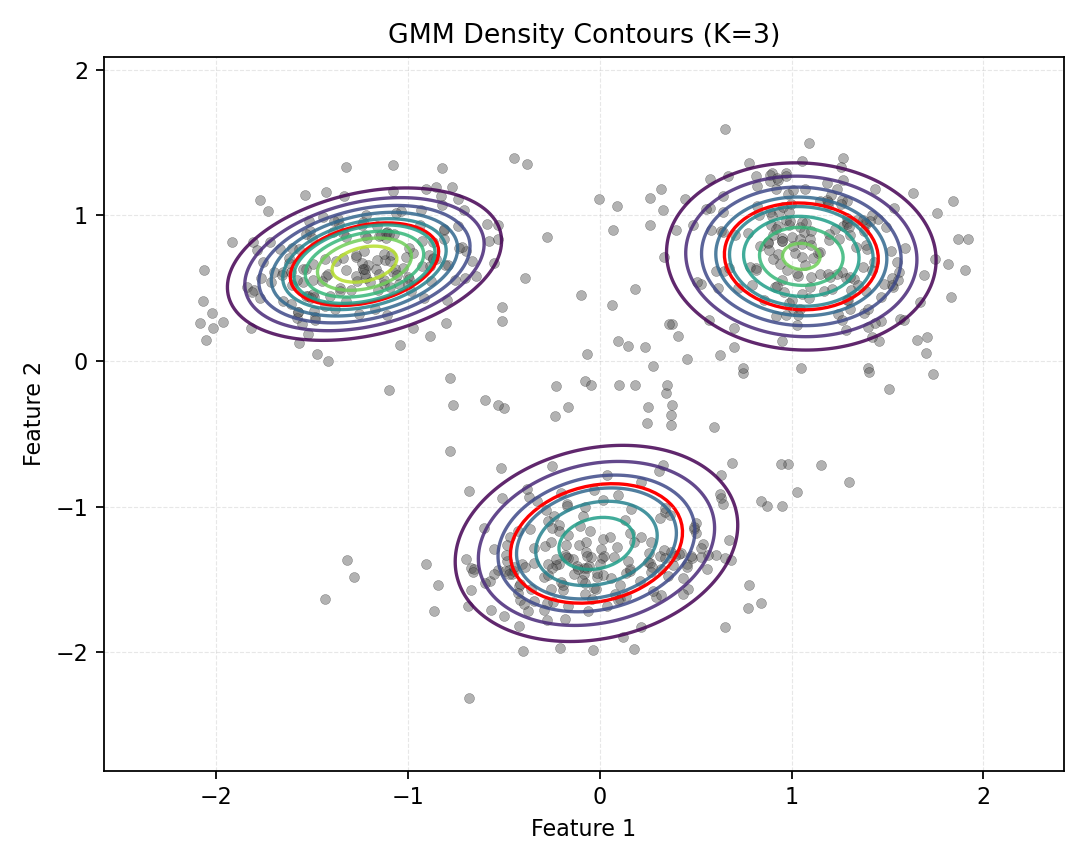
\includegraphics[width=0.82\linewidth]{gmm_density_contours.png}
  \caption{Density contours from a three-component GMM fitted to synthetic data}
  \label{fig:gmm_density_contours}
\end{figure}

\begin{figure}[H]
  \centering
  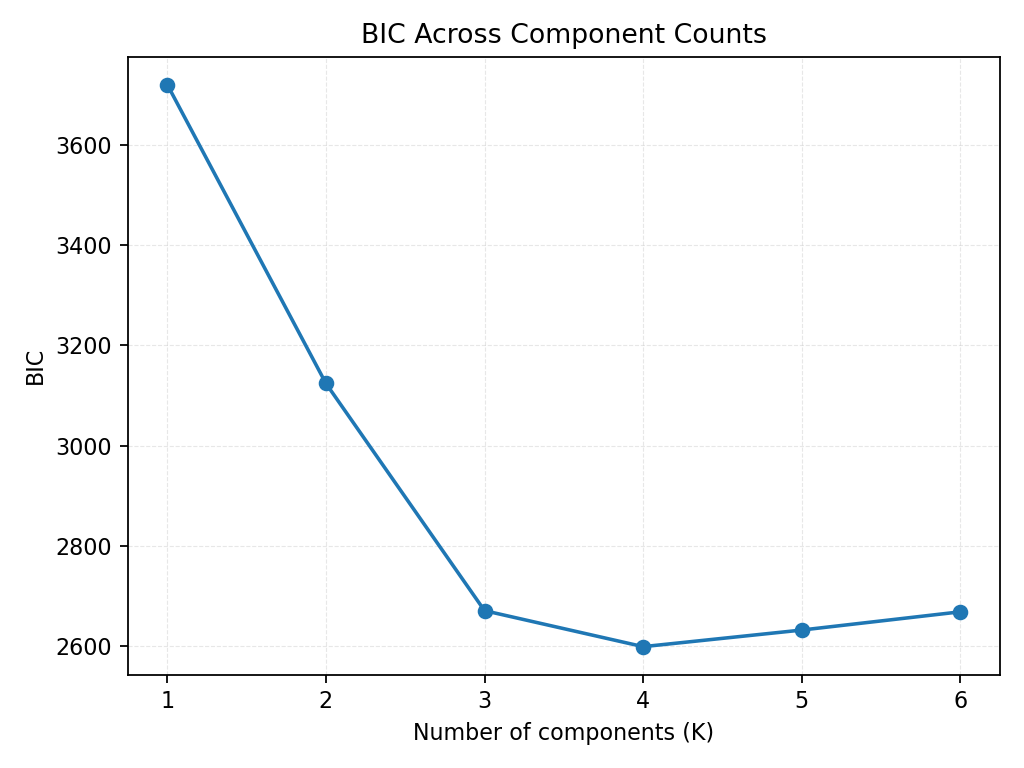
\includegraphics[width=0.8\linewidth]{gmm_bic_curve.png}
  \caption{BIC across candidate component counts}
  \label{fig:gmm_bic_curve}
\end{figure}

\FloatBarrier
\section{Summary}
Gaussian Mixture Models generalize K-means by modeling covariance structure and providing probabilistic assignments. EM alternates between computing responsibilities and updating parameters until convergence. Diagnostics such as BIC and likelihood surfaces help tune component counts and detect degenerate solutions. The synthetic example highlights how density visualization and model selection complement each other in practice.

\end{document}
